\documentclass{article}
\usepackage[margin=1.0in]{geometry} % smaller margin for document
\usepackage[margin=.7in]{caption} % little more margin for captions to make look nice
\usepackage{graphicx}
%\usepackage[export]{adjustbox}   % drop unused package

\title{The effect of pipeline-collection-diversity on performance}

\author{Sean Carver @ Data Machines Corporation}

\begin{document}

\maketitle

\abstract{Do performers who submit \emph{diverse} collections of
  pipelines tend to perform better than those who submit less diverse
  collections of pipelines?  The answer for the Winter 2020 evaluation
  is: \emph{effectively no, while technically yes.} More precisely,
  while there does exist a measurable (i.e.\ significant) improvement
  in best score with increasing diversity, the effect-size is small
  enough that it should not be of any consequence for making
  recommendations to performers.}

\section{Introduction}
In section \ref{sec:measures}, \emph{Measures of Diversity}, we define
several measures of the diversity within a collection of three or more
pipelines.

In section \ref{sec:glance}, \emph{Results at a Glance}, we present a
heat map showing briefly the (weak) connection between diversity and
performance.

In section \ref{sec:significant}, \emph{The effect is significant}, we
show that diversity has a significant effect on performance.

In section \ref{sec:small}, \emph{The effect is small}, we justify the
statement that the effect is small for the evaluation under
consideration, Winter 2020.

In a final section \ref{sec:visualization}, \emph{Visualizing
  collections} we show a cartoon visualization of collections of
pipelines for a problem together with a multiple alignment.

\section{Measures of Diversity}
\label{sec:measures}
Before we can define \emph{diversity} of a collection of (say 3 to 20)
pipelines, we first need to define the distance between two pipelines.
We choose the Levenshtein edit distance as this measure between two
pipelines.  Specifically, we first express the pipelines as sequences
of primitives, where primitives are written as ``letters'' in a large
alphabet.  The software we use accommodates all D3M primitives with
two letter pairs, each pair representing a single ``letter''
(primitive) of the alphabet.  The Levenshtein edit distance is the
minumum number of substitutions, insertions and/or deletions needed to
bring one sequence to coincide with the other.  This measure satisfies
the axioms for a distance.

But distance involves just two pipelines; diversity measures variation
among a collection of three or more pipelines.  We tried several
alternatives for quantifying diversity.  The most well-behaved
measures (i.e.\ the ones that behave most closely to our expectations
on synthetic data) were vector norms where the vector components were
the Levenshtein distances for all possible unordered pairs of
pipelines in the collection.

More precisely, we used $l_p$ norms where $p$ was a parameter varying
between 1 and $\infty$.  The different norms measure different
quantities.  At the extreme, the $l_\infty$ norm (maximum
edit-distance component) is large when there is at least one pair of
pipelines at great distance, regardless of the positions (great or
small) of the other as-close or closer distances.  On the other hand,
the $l_1$ norm (sum of the edit-distance components) can still be
relatively large if there are many pairs pipelines at moderate
distance, even though there is no pair at great distance.  We point
out that the choice the different norms can sometimes matter: we have
noted that the choice can order sets of collections---synthetic or
real---differently in terms of diversity.

Note that absolute values found in textbook definitions of the $l_p$
norm:
$$l_p([v_1,\dots,v_n]) = \sqrt[p]{|v_1|^p + \dots + |v_n|^p}$$ remain
unnecessary because all distances (e.g.\ the Levenshtein edit distance
components of $v$) must be non-negative by the properties of distance.

In the $l_p$ norm, what value for the parameter $p$ do we pick?  If
you are using only one measure of diversity, we recommend the $l_2$
norm as a nice tradeoff between the two extremes.  That said, it is
more informative to report two or more measures of diversity, in which
case $l_1$ and $l_\infty$ should be included because they are most
independent.

\section{Results at a Glance}
\label{sec:glance}
We showed the $l_2$ measure of diversity together with an indication
of best for problems, across performer and problem category.  See
Figure \ref{fig:heatmap}.  The figure suggests, as we have stated in
the abstract, a small but measurable effect of diversity on
performance.

% the [h] asks LaTeX to keep the image Here
\begin{figure}[h]
% typically cenetered
\centering
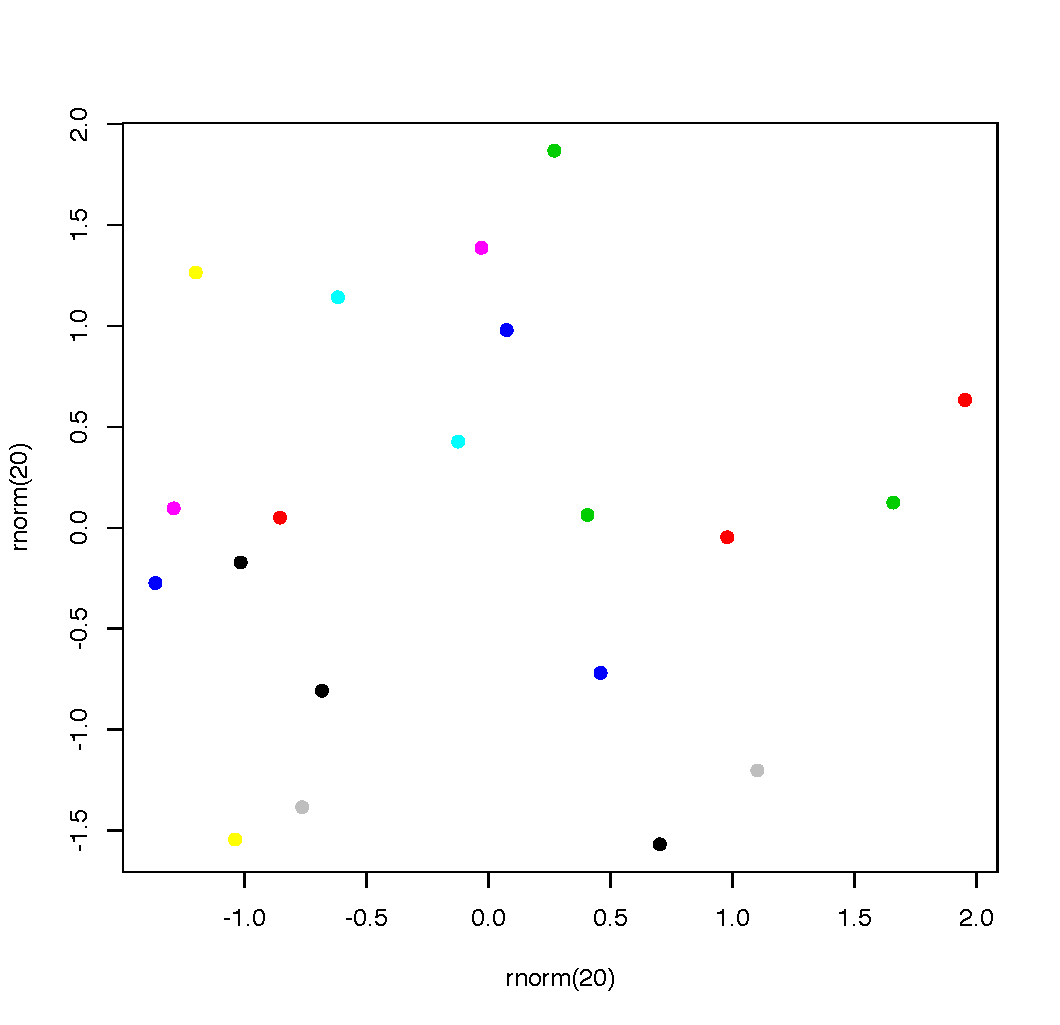
\includegraphics[scale=.6]{heatmap.pdf}
\caption{Heat map of $l_2$ diversity see section ``Measures of
  Diversity'' for a discussion of this and other measures we use to
  quantify diversity.  The horizontal axis is the problem category and
  the vertical axis is performer for the Winter 2020 evaluation.  The
  number of asterisks in each cell is the number of problem instances
  in the corresponding category-performer which was the best (or tied
  for best) performing pipeline for any problem.  There were 37 ties
  (including multi-way ties), corresponding to an additional 37
  asterisks in the figure beyond the total number of 103 problems.}
\label{fig:heatmap}
\end{figure}

\section{The effect is significant}
\label{sec:significant}
We claim that the effect of diversity on the Winter 2020 evaluation
was measurable, meaning statistically significant.

\section{The effect is small}
\label{sec:small}
We claim that the effect size is small enough that it may be
inconsequential.

\section{Visualizing collections}
\label{sec:visualization}
In this final section, we show a cartoon visualization of collections
of pipelines for a problem together with a multiple alignment.

\end{document}


  
